\documentclass{article}
\usepackage[a3paper,landscape]{geometry}
\usepackage[brazil]{babel}
\usepackage{graphicx}
\usepackage[utf8]{inputenc}
\usepackage{sectsty}
\usepackage{longtable}
\usepackage{subfigure}
\usepackage{adjustbox}
\usepackage[table]{xcolor}    % loads also colortbl
\title{ Teoria da Computação 2024/2}
\date{}
\author{ prof. Daniel Saad}
\allsectionsfont{\centering}
    
\begin{document} \maketitle
    \rowcolors{2}{white}{gray!25}
    \begin{longtable}{|l|c|c|c|c|}
    \hline
Matrícula & Prova 1 & Prova 2 & Prova 3 & Nota Final\\\hline \endhead   
141057600003 & 6.0 & - & - & -\\\hline
151057600003 & - & - & - & -\\\hline
151057600064 & 1.0 & - & - & -\\\hline
161057600019 & 2.9 & - & - & -\\\hline
181057600016 & 9.6 & - & - & -\\\hline
181057600036 & 8.4 & - & - & -\\\hline
181057600048 & 2.3 & - & - & -\\\hline
181057600051 & - & - & - & -\\\hline
181057600065 & 1.9 & - & - & -\\\hline
191057600048 & 6.9 & - & - & -\\\hline
191057600056 & 4.1 & - & - & -\\\hline
191057600059 & 10.0 & - & - & -\\\hline
201057600022 & 3.9 & - & - & -\\\hline
201057600023 & 4.9 & - & - & -\\\hline
201057600038 & 1.2 & - & - & -\\\hline
201057600040 & - & - & - & -\\\hline
201057600041 & 5.7 & - & - & -\\\hline
201057600046 & 1.0 & - & - & -\\\hline
201057600052 & 1.5 & - & - & -\\\hline
201057600056 & 6.0 & - & - & -\\\hline
201057600058 & - & - & - & -\\\hline
201057600061 & - & - & - & -\\\hline
201057600065 & - & - & - & -\\\hline
211057600022 & 7.9 & - & - & -\\\hline
211057600026 & 8.4 & - & - & -\\\hline
211057600029 & 4.4 & - & - & -\\\hline
211057600034 & - & - & - & -\\\hline
211057600035 & - & - & - & -\\\hline
211057600041 & - & - & - & -\\\hline
211057600071 & 7.0 & - & - & -\\\hline
212057600001 & 1.5 & - & - & -\\\hline
221056610016 & 0.7 & - & - & -\\\hline
221057600020 & 0.8 & - & - & -\\\hline
221057600024 & - & - & - & -\\\hline
221057600038 & - & - & - & -\\\hline
221057600047 & - & - & - & -\\\hline
221057600053 & 3.2 & - & - & -\\\hline
221058100021 & 1.4 & - & - & -\\\hline
231056610010 & 8.2 & - & - & -\\\hline
231057600001 & 7.6 & - & - & -\\\hline
231057600002 & 10.0 & - & - & -\\\hline
231057600005 & 9.4 & - & - & -\\\hline
231057600007 & 9.6 & - & - & -\\\hline
231057600009 & 10.0 & - & - & -\\\hline
231057600013 & 6.7 & - & - & -\\\hline
231057600018 & 8.8 & - & - & -\\\hline
231057600023 & 5.1 & - & - & -\\\hline
231057600025 & 3.9 & - & - & -\\\hline
231057600027 & 1.2 & - & - & -\\\hline
231057600031 & 5.7 & - & - & -\\\hline
231057600033 & 4.5 & - & - & -\\\hline
231057600034 & 10.0 & - & - & -\\\hline
231057600037 & 5.9 & - & - & -\\\hline
231057600040 & 10.0 & - & - & -\\\hline
231057600042 & 9.2 & - & - & -\\\hline
231057600044 & 1.2 & - & - & -\\\hline
231057600047 & - & - & - & -\\\hline
231057600048 & 0.8 & - & - & -\\\hline
231057600051 & 5.6 & - & - & -\\\hline
231057600054 & - & - & - & -\\\hline
231057600058 & - & - & - & -\\\hline
231057600059 & 1.5 & - & - & -\\\hline
241057600030 & - & - & - & -\\\hline
242057600002 & - & - & - & -\\\hline
\end{longtable}
\begin{figure}[h!]
\centering\begin{subfigure}
        \centering
        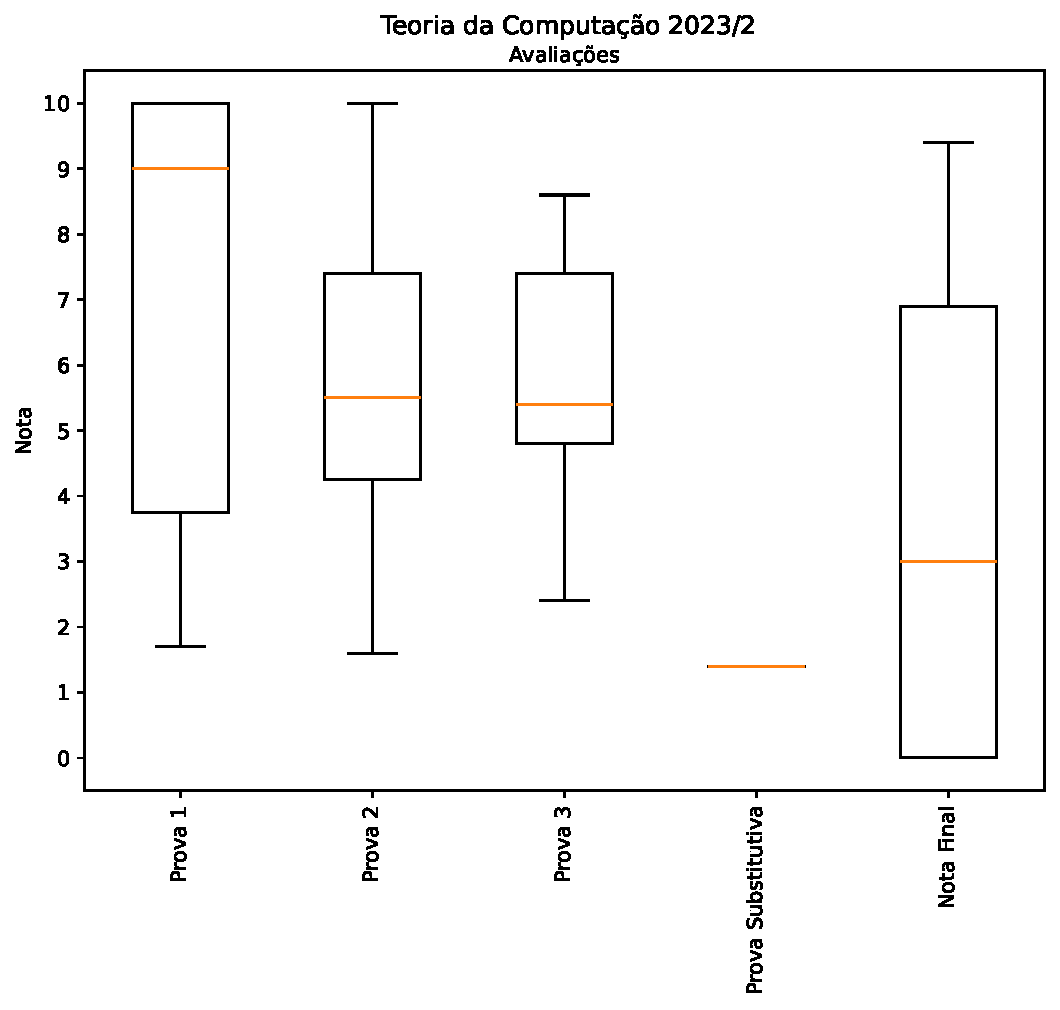
\includegraphics[width=.8\textwidth]{/home/danielsaad/git/ifb/disciplinas/teoria-da-computacao/assets/boxplot.pdf}
    \end{subfigure}\end{figure}\end{document}
